\documentclass{beamer}

\usepackage{float, graphicx}
\usepackage{listings}
\usepackage{xcolor}
\usepackage{amsthm}
\usepackage{ctex}

\lstset{
    columns = fixed,
    basewidth = {0.5em},
    % numbers = left,
    breaklines = true,
    backgroundcolor = \color{white},
    keywordstyle = \color[RGB]{40, 40, 255},
    numberstyle = \footnotesize\color{darkgray},
    commentstyle = \ttfamily\color{violet},
    basicstyle = \small\ttfamily,
    stringstyle = \ttfamily\color[RGB]{128, 0, 0},
    showstringspaces = false,
    language = {[11]C++},
}

\lstnewenvironment{cpp}{\lstset{language = {[11]C++}}}{}

\newcommand{\red}[1]{\textcolor{red}{#1}}
\newcommand{\blue}[1]{\textcolor{blue}{#1}}
\newcommand{\gray}[1]{\textcolor{gray}{#1}}
\newcommand{\teal}[1]{\textcolor{teal}{#1}}

\renewcommand{\bf}[1]{\textbf{#1}}
\newcommand{\ttt}[1]{\texttt{#1}}
\newcommand{\bluett}[1]{\blue{\ttt{#1}}}
\newcommand{\redtt}[1]{\red{\ttt{#1}}}

\newcommand{\new}{\bluett{new}~}
\newcommand{\const}{\bluett{const}~}
\newcommand{\auto}{\bluett{auto}~}
\newcommand{\struct}{\bluett{struct}~}
\newcommand{\class}{\bluett{class}~}
\newcommand{\this}{\bluett{this}~}
\newcommand{\public}{\bluett{public}~}
\newcommand{\private}{\bluett{private}~}
\newcommand{\virtual}{\bluett{virtual}~}
\newcommand{\override}{\bluett{override}~}

\usetheme{CambridgeUS}

\title{CS100 Recitation 9}
\author{Dinghao Cheng}
\date{May 10, 2022}

\AtBeginSubsection{
    \begin{frame}{Contents}
        \tableofcontents[currentsection, currentsubsection]
    \end{frame}
}

\begin{document}

\begin{frame}
    \maketitle
\end{frame}

\begin{frame}{Contents}
    \tableofcontents
\end{frame}

\section{Review on Containers}

\subsection{Container ctors}

\begin{frame}[fragile]{Container ctors}
    All STL containers support this 4 ctors (\bluett{vector} as example):
    \begin{cpp}
std::vector<Type> c; // default-initialization
std::vector<Type> c(c2); // c2 also vector, with the same <Type>
std::vector<Type> c = {a,b,c,d}; // initializer-list, container size determined by # of arguments
std::vector<Type> c(it1,it2); // copy of elements between this 2 iterators, the type of elements must be consistent with <Type>
    \end{cpp}
    Only Sequential Containers (except \bluett{std::array}):
    \begin{cpp}
std::vector<Type> c(n); // n elements, value-initialization
std::vector<Type> c(n,value); // n elements of value
    \end{cpp}
\end{frame}

\subsection{Assotiative containers}

\begin{frame}[fragile]{Assotiative containers}
    \begin{itemize}
        \item \bluett{std::map, std::set, std::multimap, std::multiset}
        \item each has according \ttt{unordered} version
        \item For map, often use together with \bluett{std::pair}.
        \item Typical usage:
    \end{itemize}
    \begin{cpp}
std::map <Keytype, Valuetype> m;
m.find(key); // return iterator to the element, end() if not found
m.count(key); // return # of elements with key
m[key] = value; // (if not exist, insert!) or update the key
    \end{cpp}
    For ordered \bf{multiple} assotiative containers,use \ttt{lower\_bound()} and \ttt{upper\_bound()} instead of \ttt{find()} to find the element with key.\\
    For unordered multiple assotiative containers, \bluett{bucket} is used.
\end{frame}

\subsection{iterators}

\begin{frame}{iterators}
    \begin{itemize}
        \item Connection between Containers and Algorithm
        \item \ttt{begin()} \ttt{cbegin()} \ttt{rbegin()} \ttt{crbegin()}\\
        \ttt{iterator} \ttt{const\_iterator} \ttt{reverse\_iterator} \ttt{const\_reverse\_iterator}
        \item \ttt{end()}: the position \bf{after the last element}
        \item Never save the value of \ttt{end()}!
        \item \ttt{insert}/\ttt{push}/\ttt{erase} may cause iterators to fail!
    \end{itemize}
\end{frame}

\begin{frame}[fragile]{range \bluett{for} statement}
    An easy and efficient way to iterate a container\\
    \begin{cpp}
for (auto& x : c) {
    // do something
};
    \end{cpp}
    \begin{itemize}
        \item c must represent a sequence (i.e. can return iterator \ttt{begin()} and \ttt{end()}).
        \item If we want to write to the elements in the sequence, the loop variable x must be a reference type.
        \item Still, we cannot add/erase elements in range for loop (this may cause iterators to fail!)
    \end{itemize}
\end{frame}

%%%%%%%%%%%%%%%%%%%%%%%%%%%%%%%%%%%%%%%%%%%%%%%%%%%%%%%%%%%%%
\section{Review on \const}

\subsection{Top-level \const Versus Low-level \const}

\begin{frame}{Top-level \const}
    \begin{itemize}
        \item Top-level \const indicates that an object \bf{itself} is \const.
        \item Top-level \const can appear in \bf{any object type}.
        \item Since a \ttt{reference} is not an object itself (do not have entity, like a ghost), it cannot have top-level \const.
    \end{itemize}
\end{frame}

\begin{frame}{Low-level \const}
    \begin{itemize}
        \item Low-level \const appears in the \bf{base type} of compound types such as \ttt{pointers} and \ttt{references}.
        \item The object pointed by the pointer / the object binded to the reference is \const.
    \end{itemize}
\end{frame}

\begin{frame}[fragile]{Low-level \const appears in the \bf{base type}}
    What is the base type?
    \begin{cpp}
typedef char *pchar;
const pchar ptr1 = NULL; 
// a const pointer pointed to char, with top-level const
// the base type is pchar, i.e. char*
const char *ptr2; 
// a pointer pointed to const char, with low-level const
// the base type is char
    \end{cpp}
\end{frame}

\begin{frame}[fragile]{Top-level \const Versus Low-level \const}
    \begin{cpp}
const int a = 1; // Top-level const, a itself is const
const int *const ptr = &a;
// const int: low-level const, the const int pointed by the pointer is const
// *const: top-level const, cannot change which int is pointed by the pointer
const int* const &p = ptr;
// a reference binded to a pointer with both top-level const and low-level const
const int *const *const ptr2 = &ptr;
// have a try?
    \end{cpp}
\end{frame}

\begin{frame}{Have some fun}
    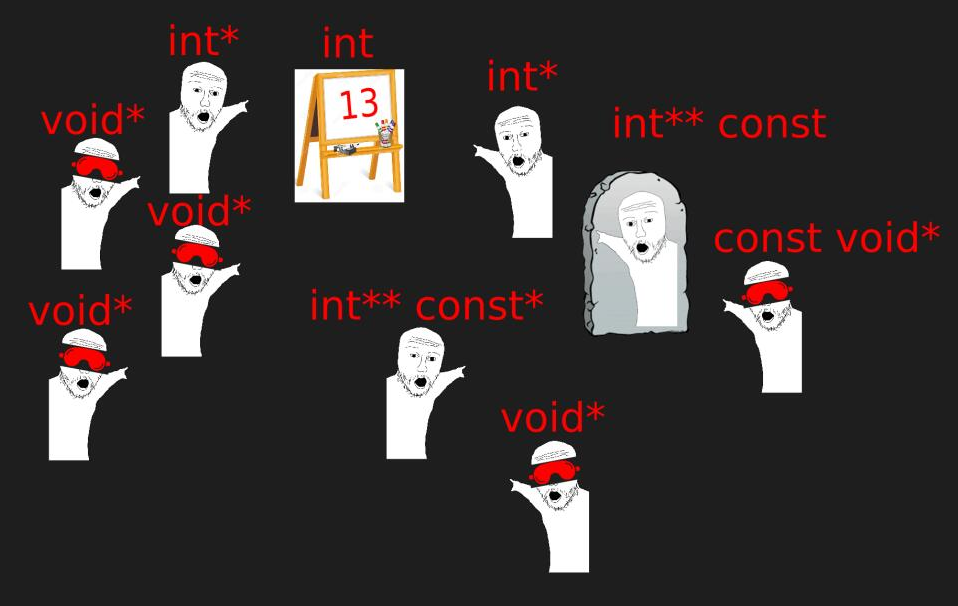
\includegraphics[width=\textwidth]{p1.png}
\end{frame}

\subsection{Type deduction in \auto}

\begin{frame}[fragile]{\auto}
    \begin{itemize}
        \item \auto ordinarily ignores top-level \const{}s.
        \item As usual in initializations, low-level \const{}s, such as when an initializer is a pointer to \const, are kept:
        \item When \auto is initialized with a reference, it will be infered as the type of the object and ignore the reference (variable c below).
    \end{itemize}
    
    \begin{cpp}
const int ci = i;
auto &cr = ci; // const int &
auto b = ci; // int (top-level const in ci is dropped)
auto c = cr; // int (cr is an alias for ci whose const is top-level)
auto d = &i; // int* (& of an int object is int*)
auto e = &ci; // const int* (& of a const object is low-level const)
    \end{cpp}
\end{frame}

\subsection{\const member function}

\begin{frame}[fragile]{Why \const overload?}
    \begin{cpp}
class Array {
public:
    // ctor, dtor, copy ctor, ...
    int &at(std::size_t n);
    const int &at(std::size_t n) const;
    // other members...
private:
    // members...
};
    \end{cpp}
    \begin{itemize}
        \item The non\const version will not be viable for \const objects; we can \bf{only} call \const member functions on a \const object.
        \item We can call either version on a non\const object, but the non\const version will be a \bf{better match}.
    \end{itemize}
\end{frame}

\begin{frame}[fragile]{Attention: return type}
    An example\\
    If we write like this...
    \begin{cpp}
class Vector {
 public:
  int &at(std::size_t n) const {
    return m_data[n];
  }
  // other members
};
    \end{cpp}
\end{frame}

\begin{frame}[fragile]{Example: Access Elements of Vector}
    \begin{cpp}
class Vector {
 public:
  int &at(std::size_t n) const {
    return m_data[n];
  }
  // other members
};
    \end{cpp}
    Still problematic:
    \begin{cpp}
const Vector v = some_value();
v.at(10) = 42;
    \end{cpp}
    Compilers may fail to detect such modification, but it is undefined behavior!
\end{frame}

\begin{frame}[fragile]{Correct Way}
    Const overloading.
    \begin{cpp}
class Vector {
 public:
  int &at(std::size_t n) {
    return m_data[n];
  }
  const int &at(std::size_t n) const {
    return m_data[n];
  }
  // other members
};
    \end{cpp}
    Calling a \const member function is actually \textbf{adding low-level \blue{const}} to the \bluett{this} pointer.
\end{frame}

\begin{frame}{Conclusion}
    Pointers and references to \const (with top-level \const): pointers or references "that think they point or refer to const."\\
    Recall: adding top-level \const and low-level \const are both \bf{safe}.\\
    Removing low level \const is \bf{dangerous}.
    \begin{alertblock}{Notice}
        \begin{quote}
            Use const whenever possible. (Effective C++, Item 3)
        \end{quote}
    \end{alertblock}
\end{frame}

%%%%%%%%%%%%%%%%%%%%%%%%%%%%%%%%%%%%%%%%%%%%%%%%%%%%%%%%%%%%%%%%%%%%%%%%%%
\section{Overload, Override and Overwrite}

\subsection{Overload}

\begin{frame}[fragile]{Overload}%/重载
    \begin{itemize}
        \item The most clearly understood one
        \item Functions(in a name lookup range) with the same name and different argument lists (and optionally different return types)
        \item Example: ctor
    \end{itemize}
    \begin{cpp}
class Point2d {
public:
    Point2d(): Point2d(0.0, 0.0) {}
    Point2d(double _x): Point2d(_x, 0.0) {}
    Point2d(double _x, double _y): x(_x), y(_y) {}
private:
    double x, y;
};
        \end{cpp}
\end{frame}

\subsection{Override}

\begin{frame}[fragile]{Override}%/覆盖
    \begin{itemize}
        \item the most clearly defined
        \item override \bf{virtual functions} in base class
        \item Example: \override specifier (Remember, when using virtual function, always write \override!)
        \item The \override keyword lets the compiler check and report if
        the function is not actually overriding. 
    \end{itemize}\begin{cpp}
class base{
public:
    virtual void f() {puts("base::f()");}
};
class derived: public base{
public:
    void f() override {puts("derived::f()");}
};
        \end{cpp}
\end{frame}

\subsection{Overwrite}

\begin{frame}[fragile]{Overwrite}%/重写(隐藏)
    \begin{itemize}
        \item Actually hide
        \item Understand with example
    \end{itemize}
\end{frame}

\begin{frame}[fragile]{Example 1:}
\begin{cpp}
class base{ public:
    virtual void f() {puts("base::f()");}
};
class d1: public base{ public:
    void f() override {puts("d1::f()");}
    void f(int a) {puts("d1::f(int)");}
    void f(double a) {puts("d1::f(double)");}
};
class d2: public d1{
};
int main(){
    d2 d;
    d.f(); // d1::f()
    d.f(3); // d1::f(int)
    d.f(3.14); // d1::f(double)
}
\end{cpp}
\end{frame}

\begin{frame}[fragile]{Example 2:}%The base member is hidden even if the functions have different parameter lists
\begin{cpp}
class base{ public:
    virtual void f() {puts("base::f()");}
};
class d1: public base{ public:
    void f() override {puts("d1::f()");}
    void f(int a) {puts("d1::f(int)");}
    void f(double a) {puts("d1::f(double)");}
};
class d2: public d1{ public:
    void f() override {puts("d2::f()");}
};
int main(){
    d2 d;
    d.f(); 
    d.f(3); //compile error!
    d.f(3.14); //compile error!
}
\end{cpp}
\end{frame}

\begin{frame}[fragile]{Example 3:}
\begin{cpp}
class base{ public:
    virtual void f() {puts("base::f()");}
};
class d1: public base{ public:
    void f() override {puts("d1::f()");}
    void f(int a) {puts("d1::f(int)");}
    void f(double a) {puts("d1::f(double)");}
};
class d2: public d1{ public:
    void f() override {puts("d2::f()");}
    using d1::f;
};
int main(){
    d2 d;
    d.f(); // d2::f()
    d.f(3); // d1::f(int)
    d.f(3.14); // d1::f(double)
}
\end{cpp}
\end{frame}

\begin{frame}{Notice}
    \begin{alertblock}{Notice}
        \begin{quote}
            Never redefine an inherited non-virtual function. (Effective C++, Item 36)
        \end{quote}
    \end{alertblock}
    \begin{itemize}
        \item Recall: polymorphism, virtual function is called according to the type of object rather than the type of pointer.
        \item Non-virtual functions are statically bound (i.e. according to the type of pointer rather than the object).
        \item This conflicts with the "is a" relationship in inheritance.
    \end{itemize}
\end{frame}

%%%%%%%%%%%%%%%%%%%%%%%%%%%%%%%%%%%%%%%%%%%%%%%%%%%%%%%%%%%%%%%%%%%%%%%%%%%
\section{Memory management}

\subsection{More on \new}

\begin{frame}[fragile]{What does \new expression do}
    \begin{cpp}
// new expressions
auto sp = new string("a value"); // allocate and initialize a string
    \end{cpp}
    \begin{enumerate}
        \item Calls a library function named \bf{operator} \new (or \bf{operator} \new []), which allocates raw, untyped memory.
        \item Run the appropriate constructor to construct the object(s) from
        the specified initializers.
        \item A pointer to the newly allocated and constructed object is returned.
    \end{enumerate}
\end{frame}

\begin{frame}[fragile]{Recall: default ctor}
    \bluett{new} not only allocates the memory, but also constructs the object (either default-initialize or value-initialize). However:
    \begin{itemize}
        \item     Some classes are designed unable to be default-initialized.
        \item Some classes may contain members that are not default-initializable.
        \item Problem: What if we want to dynamically allocate memory for these class members?
    \end{itemize}
    \begin{cpp}
        auto p = new MyClass[10](233); // Compile error!
    \end{cpp}
    Array \bluett{new} cannot have initialization arguments.\\
    (Even though, you can use braced initializer list when there is constexpr number of elements.)
\end{frame}

\begin{frame}[fragile]{\bf{placement} \new}
    If \ttt{placement-params} are provided, they are passed to the allocation function as additional arguments. Such allocation functions are known as "\bf{placement} \new".\\\begin{cpp}
new (place_address) type (initializers)
new (place_address) type [size] {braced initializer list}
    \end{cpp}
    \bf{placement} \new is used to construct objects in allocated storage (even on the stack, e.g. in a \bluett{union}).
\end{frame}

\subsection{Allocator}

\begin{frame}[fragile]{Allocator}
    \begin{itemize}
        \item \bluett{allocators} allocates unconstructed memory, lets us separate allocation from construction.
        \item We must \ttt{construct} objects in order to use memory returned by
        \bluett{allocate}. Using unconstructed memory in other ways is undefined behavior!
        \item \ttt{std::allocator} object has method \bluett{allocate}, \bluett{deallocate} (\bluett{construct}, \bluett{destroy} are deprecated in C++17, they are just encapsulation of placement \new and dtor call).
        \item \ttt{allocator\_traits} instead, is used in most of the STL containers.
        \item Usage:
    \end{itemize}
\end{frame}

\begin{frame}[fragile]{\ttt{std::allocator::allocate()}}
    \begin{itemize}
        \item Return a pointer to the start address of the allocated memory.
        \item Compared to directly calling operator \bluett{new}, the allocator may use some optimization, such as memory pool in SGI.
    \end{itemize}
    \begin{cpp}
        std::allocator<MyClass> alloc;
        auto p = alloc.allocate(10); // actual type: MyClass*
    \end{cpp}
\end{frame}


\begin{frame}[fragile]{\ttt{std::allocator::construct()}}
    (Deprecated in C++17)\\
    Accept one or multyple arguments which are passed to the ctor of the class.\\
    Actually calling placement \new.
    \begin{cpp}
        std::allocator<MyClass> alloc;
        auto p = alloc.allocate(10); // actual type: MyClass*
        auto q = p;
        for (int i=0; i<10; ++i){
            // alloc.construct(q++, i);
            new(q++) MyClass(i);
        }
    \end{cpp}
\end{frame}

\begin{frame}[fragile]{\ttt{std::allocator::destroy()}}
    (Deprecated in C++17)\\
    We may \bluett{destroy} only elements that are actually \bf{constructed}!\\
    Actually calling dtor.
    \begin{cpp}
        std::allocator<MyClass> alloc;
        auto p = alloc.allocate(10); // actual type: MyClass*
        auto q = p;
        for (int i=0; i<10; ++i)
            new(q++) MyClass(i);
        q = p;
        for (int i=0; i<10; ++i)
            // alloc.destroy(q++, i);
            (q++)->~MyClass();
    \end{cpp}
\end{frame}

\begin{frame}[fragile]{\ttt{std::allocator::deallocate()}}
    The pointer we pass to deallocate cannot be null; it must point to memory allocated by allocate.\\
    Moreover, the size argument passed to deallocate must be the same size as used in the call to allocate that obtained the memory to which the pointer points.
    \begin{cpp}
        std::allocator<MyClass> alloc;
        auto p = alloc.allocate(10); // actual type: MyClass*
        auto q = p;
        for (int i=0; i<10; ++i)
            new(q++) MyClass(i);
        q = p;
        for (int i=0; i<10; ++i)
            (q++)->~MyClass();
        alloc.deallocate(p, 10);
    \end{cpp}
\end{frame}

\end{document}